\chapter{Performance analysis}\label{ch:results}
% Validation: Are we building the right system?
% Verification: Are we building the system right?
To analyze how feasible is it to run all Tribler functionality on mobile devices, we measure several performance characteristics relevant to the functional and non-functional requirements in Chapter \ref{ch:design}.
We take several measurements on different devices to quantify the performance and resource usage in the context of the scenario in the problem description in Chapter \ref{ch:problem_desc}.
The results will indicate the state of the art, before any optimization, in functionality of Tribler on mobile devices as described in Chapter \ref{ch:tribler}.
From the results, possible angles for optimization will emerge and further described in Chapter \ref{ch:conclusions}.

% Rationale
% Metrics
% Expected / desired results
% Setup
% Results
% Conclusions

\section{Content discovery}\label{sec:content_discovery}
% Rationale
Before anyone can view new content that has been added to a channel, it needs to be discovered by other devices.
% Metrics
We measure the amount of time it takes for other devices to discover new content in a channel they are subscribed to, starting from the moment it is added to that channel.
% Expected / desired results
Depending on the random walk in the channel's community content can be discovered either very quickly or after a while due to property of eventual consistency.
% Setup
\begin{figure}[H]
	\centering
	\includegraphics[width=\textwidth]{phones_2}
	\caption{Experimental setup with various smartphones and one tablet, all showing the About Android screen.}
	\label{fig:phones_2}
\end{figure}

\begin{table}[H]
	\begin{tabular}{l | *{6}{c} || c} \hline
		Device & Nexus 5 & Nexus 6 & Galaxy Nexus & Galaxy S3 & OnePlus One & Nexus 10 & Total \\ \hline
		Amount & 1 & 4 & 6 & 1 & 1 & 1 & 14 \\ \hline
	\end{tabular}
	\caption{Devices used in the content discovery experiment.}
	\label{table:devices}
\end{table}

Figure \ref{fig:phones_2} shows the experimental setup with various smartphones and one tablet.
Each device is connected to the same wireless network and within 1 to 2 meters distance from the same access point.
Different versions of Android OS are installed, ranging from 4.3 to 7.1, and some run a CyanogenMod.
Each device is installed with the same version of Tribler and the same database, containing up to date information about existing channels and their content.
This database was gathered in the days before this experiment, serving as a hot cache.
On one device, a Nexus 6, from now on referred to as the source, a new channel is created to which the other 13 devices subscribe via NFC.
Then, repeatedly a new video is recorded and added to that channel by the source.
The new videos are discovered, and the event logged, by each device individually.
\begin{figure}[H]
	\centering
	\includegraphics[width=.8\textwidth]{content_dissemination}
	\caption{Sequence of events when a video is recorded and distributed.}
	\label{fig:content_dissemination}
\end{figure}
The sequence, as shown in Figure \ref{fig:content_dissemination}, of recording a new video, adding it the the same channel, and letting the subscribers discover it, is repeated 15 times for accuracy.
All devices are synced with NTP to be able to have a common timeline for this experiment.

% Results
\begin{figure}[H]
	\centering % trim={<left> <lower> <right> <upper>}
	\includegraphics[trim={0.9cm 0 0 0},clip,width=\textwidth]{boxplot-nrofdevices-130}
	\caption{Elapsed time after adding new content to a channel and it being discovered by subscribed peers.}
	\label{fig:boxplot-nr.of.devices-130}
\end{figure}
Figure \ref{fig:boxplot-nr.of.devices-130} shows the amount of time it takes a number of devices to discover new content on a subscribed channel.
The results show that the first device discovers new content in less than 2 seconds, while within 4 seconds 9 devices have discovered the new content.
From the 10th device and beyond an increase in discovery time is noticeable.
% Conclusions
This could be explained by the fact that only 10 peers are connected at a time.
Many more peers are needed to give an accurate representation in terms of scalability.
What can be concluded from this experiment is that on the same local network the first device discovers the new content in less than 2 seconds.
From the 10th device onward the dissemination slows down.


\section{Multichain performance}\label{sec:multichain_perf}
% Rationale
If mobile devices are to become full-fledged nodes on the network they must support the Multichain feature.
% Metrics
The creation and signing of these blocks is measured to determine if it scales well.
Multichain signs a block every 10 minutes, meaning our experiment of generating 25,000 blocks represent about half a year (173.6 days) of continuous effort.
% Expected / desired results
The database containing these blocks will grow over time, but should not slow down too much because of it.
% Setup
Measurements were taken on six different devices on multiple moments during development.
A laptop is included to give some more perspective.
Its specifications are listed in Table \ref{table:specs_laptop}.
% Results
Figure \ref{fig:multichain_25} shows the performance graphs of every measurement.
\begin{figure}[H]
	\centering
	\includegraphics[width=\textwidth]{multichain_scale_2599_25k}
	\caption{Creating and signing of 25,000 blocks between two peers}
	\label{fig:multichain_25}
\end{figure}
\begin{table}[H]
	\begin{tabular}{l | l} \hline
		Laptop & Dell Latitude E6520 \\ \hline \hline
		CPU & i7-2760QM @ 2.4GHz \\ \hline
		RAM & 8 GB @ 1333 MHz \\ \hline %% NT4GC64B8HG0NS-CG
		SSD & 80GB X25-M \\ \hline %% SSDSA2M080G2GC
	\end{tabular}
	\caption{Hardware specifications of the laptop used in the Multichain and API measurements.}
	\label{table:specs_laptop}
\end{table}
Clearly visible from the graphs is that Multichain does not scale linearly on any device.
They also show that mobile devices are at least a factor of two slower than an ordinary laptop and scale worse.
% Conclusions
Due to the nature of blockchain every new block needs to contain the hash value of the previous block.
If a database lookup is needed for this and the database is growing, that can explain the non-linear course of the graph.
This can be easily optimized by keeping the last hash value for currently connected peers in memory.
However this is an indication that creating blocks by the thousands is an IO bound process, rather than CPU bound.
Finally, if mobile devices are to be full-fledged nodes on the Tribler network, they should not slow down significantly more than any other ordinary laptop, besides being slower in the first place.
Hardware acceleration could close this gap without sacrificing battery life too much.
Because mobile devices are a bit behind on the technology curve with respect to desktop computers it is probable that the gap becomes smaller over the coming years.
The capacity to store enough Multichain blocks to audit past exchanges should also be on par.
If not, other more powerful nodes could be queried to supply the necessary history about a peer, that requests your bandwidth, to verify if that peer is trustworthy.


\section{Startup time}\label{sec:startup_time}
%TODO previous chapter: implementation architecture startup sequence nice design, how does it perform?
% Rationale
Key to user retention is a fast startup time.
The app starts the GUI first, followed by the service.
Loading of the GUI is fast, because it is in fact a thin shell, thanks to the separation of the back-end and the front-end, and the asynchronous implementation.
This enables the GUI to be visible and responsive to user input, as shown in Figure \ref{fig:menu-popular}, while the service may continue loading in the background.
However, before any task can be executed by the service, it needs to be fully started.
% Metrics
To measure the total startup time we register the time of launching the app and the moment the Tribler-started-event is registered by the GUI.
This event is sent over the API event-stream and indicates that the service is fully started and ready to accept all incoming requests.
% Expected / desired results
We expect consistent loading times on each device, and potentially significant different loading times between devices, because of differences in hardware.
% Setup
Therefore, we measure the startup time 10 times on 5 different devices.
The app is launched with Android Debug Bridge (ADB) from a laptop and the Tribler-started-event is read directly from the device's log over ADB and timed on the same laptop, so they use the same clock.
% Results
\begin{figure}[H]
	\centering % trim={<left> <lower> <right> <upper>}
	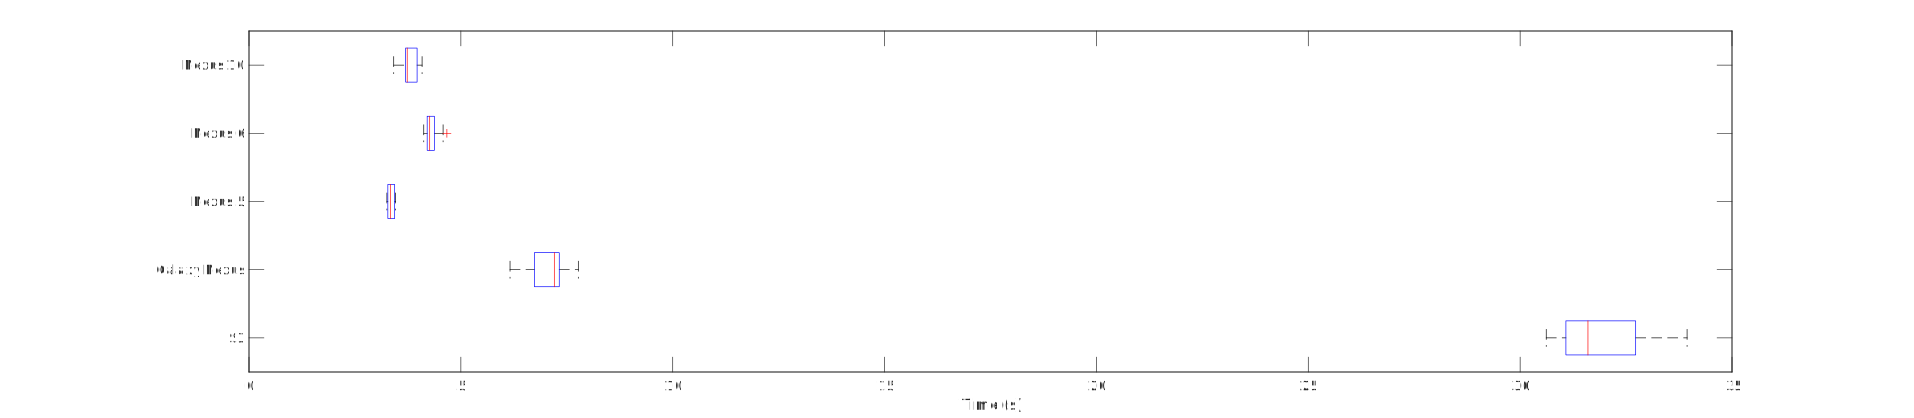
\includegraphics[trim={4cm 0cm 4cm 0cm},clip,width=\textwidth]{boxplot-startup}
	\caption{Startup time per device for 10 consecutive runs.}
	\label{fig:boxplot-startup}
\end{figure}
\begin{table}[H]
	\begin{tabular}{l | *{5}{r}} \hline
		Device & N & Avg. (s) & Min. (s) & Max. (s) & s (s) \\ \hline \hline
		Nexus 10        & 10 & 3.781 & 3.416 & 4.085 & 0.211 \\ \hline
		Nexus 6          & 10 & 4.319 & 4.124 & 4.670 & 0.179 \\ \hline
		Nexus 5          & 10 & 3.353 & 3.273 & 3.459 & 0.081 \\ \hline
		Galaxy Nexus & 10 & 7.086 & 6.161 & 7.772 & 0.454 \\ \hline
		S3                   & 10 & 31.935 & 30.616 & 33.940 & 1.116 \\ \hline
	\end{tabular}
	\caption{Statistics of startup time per device.}
	\label{table:startup_time}
\end{table}
Table \ref{table:startup_time} shows the statistics per device.
The results show a very small sample standard deviation and a very low startup time.
The S3 is performing way worse than may be expected from comparing the results of the other devices and the Multichain experiment.
% Conclusions
The reason for that may be that this phone was not wiped and given a fresh install of Android before starting the experiment like the other devices were.
Which would mean that other applications installed on a device could significantly impact the startup performance of Tribler.
This should be investigated further, including if anything can be done on the part of Tribler.
The sample standard deviation is relatively small for all devices, which indicates that the startup time of Tribler is consistent.


\section{Content creation}\label{sec:content_creation}
%TODO grote scenario
% Rationale
New content can be generated with a smartphone, like for example a video that has been recorded with the built-in camera.
How quick one can create content and distribute it depends not only on the discovery time, as measured in Section \ref{sec:content_discovery}, but first, and perhaps foremost, on the speed of the torrent creation process.
% Metrics
In this experiment we measure the time required to create a torrent file for different sizes of videos.
We also measure the amount of time it takes to add that torrent to a channel.
% Expected / desired results
In the torrent creation process a hash is calculated for each piece of the content.
Therefore, the amount of time it takes for a torrent to be created is relative to the size of the content.
Because this is a CPU intensive task, we expect the time required to create a torrent file to follow the time complexity of the hash function.
% Setup
The setup for this measurement is exactly the same as in Section \ref{sec:content_discovery}, but we only look at the source, creating and adding the torrent of the video content.
% Results
Figure \ref{fig:scatterplot-torrent-create} shows the relation between the size of the content and the time required to create a torrent file for it.

\begin{minipage}{.49\textwidth}
\begin{figure}[H]
	\centering % trim={<left> <lower> <right> <upper>}
	\includegraphics[trim={3cm 7cm 3cm 7.5cm},clip,width=\textwidth]{scatterplot-torrent-create}
	\caption{Creating a torrent for content of varying size.}
	\label{fig:scatterplot-torrent-create}
\end{figure}
\end{minipage}
~
\begin{minipage}{.49\textwidth}
\begin{figure}[H]
	\centering % trim={<left> <lower> <right> <upper>}
	\includegraphics[trim={3cm 7cm 3cm 7.5cm},clip,width=\textwidth]{scatterplot-torrent-add}
	\caption{Adding a torrent to a channel for content of varying size.}
	\label{fig:scatterplot-torrent-add}
\end{figure}
\end{minipage}

% Conclusions
The results suggest a linear correlation between the size of a video and the torrent creation time, with one outlier in this set of eight samples.
However, due to differences in hardware acceleration of the hashing algorithm implementation and small amount of data, no claims can be made in general.
% is very large with respect to the data points
Finally, to add content to a channel, only metadata is required, which does not scale with content size, as can be seen in Figure \ref{fig:scatterplot-torrent-add}.
However, the margin of error is also determined by the API response time, which we will measure in the next section.


\section{API responsiveness}\label{sec:api_responsiveness}
% Rationale
By design most functionality is operated through the API.
% Metrics
Therefore, measuring the responsiveness of the API will give a good indication of the responsiveness overall.
We use Apache JMeter to fire requests at the API and measure the time it takes to respond to each request.
JMeter's 'latency' metric measures the time from just before sending the request, to just after the first part of the response has been received \cite{jmeter_glossary}.
Thus, this metric includes the following:\\
\begin{minipage}{\textwidth}
\hspace{13em}
\begin{minipage}{.5\textwidth}
\emph{
	time needed to assemble the request by the client\\
	+ time to connect to the server\\
	+ latency towards the serve\\
	+ time for processing the request by the server\\
	+ time to generating a response by the server\\
	+ latency back from the server.\\
}
\end{minipage}
\end{minipage}
It excludes the transfer time of the complete response, and subsequent processing and rendering time by the client, because any client can do so differently, for example in a streaming fashion.
% Expected / desired results
We want to see that the response time is bounded, consistent and generally low.
% Setup
A Nexus 6 smartphone with Android 7.1 CyanogenMod is connected to a laptop running JMeter and the API port is forwarded with ADB over USB2.0.
With JMeter we request the discovered channels from the API a 1,000 times at a constant rate of one request per second sequentially.
A laptop is included to give some more perspective.
Its specifications are listed in Table \ref{table:specs_laptop}.
The measurements are repeated for two scenarios: at first launch, and when almost no new channels are discovered anymore.
% Results
Figure \ref{fig:api_combined} shows the response times and sizes for every request in both scenarios for the laptop and Nexus 6 smartphone.
\begin{figure}[H]
	\centering
	\begin{subfigure}{.49\textwidth}
		\includegraphics[width=\textwidth]{api_combined_Laptop}
		\caption{Laptop, at first launch}
		\label{fig:api_Laptop}
	\end{subfigure}
	~
	\begin{subfigure}{.49\textwidth}
		\includegraphics[width=\textwidth]{api_combined_Nexus_6}
		\caption{Nexus 6 smartphone, at first launch}
		\label{fig:api_Nexus_6}
	\end{subfigure}
	
	\begin{subfigure}{.49\textwidth}
		\includegraphics[width=\textwidth]{api_combined_Laptop-2}
		\caption{Laptop, after most channels are discovered}
		\label{fig:api_Laptop-2}
	\end{subfigure}
	~
	\begin{subfigure}{.49\textwidth}
		\includegraphics[width=\textwidth]{api_combined_Nexus_6-2}
		\caption{Nexus 6 smartphone, after most channels are discovered}
		\label{fig:api_Nexus_6-2}
	\end{subfigure}
\caption{API response times (black) and sizes (red) for a 1,000 requests, to return all discovered channels, at first launch (top), and when almost no new channels are discovered anymore (bottom)\\
N.B. Response time is measured up to the moment the first part of a response has been received, therefore the transfer time of the entire response is not included}
\label{fig:api_combined}
\end{figure}
\begin{table}[H]
  \begin{tabular}{l | *{8}{r}} \hline
  	  & N & Avg. (ms) & Min. (ms) & Max. (ms) & $\sigma$ (ms) & Req./min. & KB/second & Avg. Bytes \\ \hline \hline
  	 Laptop   & 1000 & 65     & 1       & 1021 & 99.00 & 60.0 & 73.72 & 75410.6 \\ \hline
  	 Nexus 6 & 1000 & 3975 & 8       & 39477 & 5362.51 & 14.4 & 49.19 & 210506.8 \\ \hline
  	 Laptop   & 1000 & 181   & 101   & 416   & 42.72   & 60.0 & 579.49 & 592791.3 \\ \hline
  	 Nexus 6 & 1000 & 1671 & 1390 & 2925 & 174.14 & 35.9 & 345.94 & 592649.8 \\ \hline
  \end{tabular}
  \caption{Statistics of API response times and sizes from Figure \ref{fig:api_Laptop}, \ref{fig:api_Nexus_6}, \ref{fig:api_Laptop-2} and \ref{fig:api_Nexus_6-2} respectively}
  \label{table:api_benchmark}
\end{table}
As shown in Table \ref{table:api_benchmark}, the smartphone achieved a considerable lower amount of requests per minute than the constant rate of one per second in both scenarios.
Therefore, because of the fixed amount of requests, proportionally more time elapsed during the measurements on the smartphone than on the laptop.
This in turn, explains the significant difference in response size at the end of the measurements at first launch between the smartphone and the laptop.
% Conclusions
The throughput of the smartphone in the second scenario is higher than the throughput of the laptop in the first scenario.
The 480 MB/s theoretical bandwidth of USB2.0 cannot be a bottleneck, considering the 579.49 KB/s result of the PC.
From this, we can conclude that bandwidth is not a limiting factor in the first scenario for the smartphone.
Although the requests are sequential, they can still influence each other, due to caching for example.
Therefore, to explain the jitter, we have to look at the internals of the Tribler core, and the environment.

Tribler uses the event-driven networking engine Twisted, which is written in Python.
Twisted allows you to build inter-process communication protocols, and provides the HTTP server used to build the REST API.
Twisted uses a single thread to coordinate all others, called the reactor thread.
If this thread is busy, the REST API can not receive incoming requests resulting in delays and potential timeouts.
Also, only one thread can be executed at a time, because our implementation uses the CPython interpreter which has a global interpreter lock (GIL).
CPython is optimized for single thread performance and compatibility with C extension modules, which are typically not thread-safe.

The fact that the smartphone in our experiment is not able to process one request per second, could indicate the multi-threaded processing capability is severely flawed due to the effects of the GIL on the Twisted reactor.
Although each measurement is a snapshot, they were taken in a short time span from each other, so the environment is not expected to have a larger impact than the aforementioned effect.
Being a mobile device also other aspects my be at play here, like CPU frequency scaling.
However, this was turned off by acquiring a wake lock from the Android OS.
There were no other active user-apps, but the OS itself contains system-apps that cannot be turned off.
Finally, the derivative of the response size appears to coincide with a significant longer response time.
If new content is discovered, that means other threads are active, which confirms our hypothesis that the GIL is to blame for poor multi-threaded performance.
Further investigation should figure out if this phenomenon is also observed with lower amounts of requests per minute, in order to determine if the CPython has to be replaced by an interpreter without a GIL.


\section{Profiling}\label{sec:profiling}
% Rationale
Because of the challenges put forward in Chapter \ref{ch:tribler_mobile} and multi-threading issues found in Section \ref{sec:api_responsiveness}, we investigate if time is spent disproportionately on some function.
% Expected / desired results
We expect that the limited resources of a mobile device may impact particular features more than others.
If hardware acceleration is not present a less powerful CPU may struggle with encryption tasks.
Long running functions impact the responsiveness due to the GIL, as explained in Section \ref{sec:api_responsiveness}.
% Metrics
We focus on wall clock time, instead of CPU time, because this metric indicates the amount of time a user has to wait for a certain function to be executed.
% Setup
With the cProfile Python module we can measure wall clock time for each function call, to see if any function takes a disproportionate amount of time.
A Nexus 6 smartphone with Android 6.0.1 CyanogenMod was used.
The profiler was running for 10 minutes, with Tribler during normal operation and without any user input.
% Results
%\begin{figure}[H]
%	\centering
%	\includegraphics[width=\textwidth]{profile_1468515157-2}
%	\caption{Profiler results of 10 minutes Tribler run time (bright pink represents business logic upon receiving a torrent)}
%	\label{fig:profile}
%\end{figure}

%The bright pink represents the update function, which signifies various business logic upon receiving a torrent.
%Also notable is the same stack of functions within and outside of a community on top of the wrapper.
%This can be explained by the fact that torrents can be discovered outside of a community too.

\begin{table}
	\begin{tabular}{r | l | l | l} \hline
		\# Calls & Total time (s) & Time per call (s) & Function \\ \hline \hline
		15 & 0.4867 & 0.03245 & method 'commit' of 'sqlite3.Connection' objects \\ \hline
		1 & 0.01692 & 0.01692 & method 'executescript' of 'sqlite3.Cursor' objects \\ \hline
		3820 & 64.28 & 0.01683 & method 'poll' of 'select.epoll' objects \\ \hline
		2 & 0.01048 & 0.005241 & \_\_m2crypto.ec\_key\_gen\_key \\ \hline
		31075 & 162 & 0.005212 & \_\_m2crypto.ecdsa\_verify \\ \hline
		1650 & 7.133 & 0.004323 & \_\_m2crypto.ecdsa\_sign \\ \hline
		1 & 0.001708 & 0.001708 & \_socket.gethostbyaddr \\ \hline
		1 & 0.001284 & 0.001284 & built-in method SSL\_library\_init \\ \hline
		567 & 0.565 & 0.0009965 & method 'executemany' of 'sqlite3.Cursor' objects \\ \hline
		8 & 0.005731 & 0.0009552 & \_\_import\_\_ \\ \hline
		12 & 0.01083 & 0.0009029 & method 'connect\_ex' of '\_socket.socket' objects \\ \hline
		1 & 0.00055 & 0.00055 & built-in method SSL\_load\_error\_strings \\ \hline
		5 & 0.002515 & 0.000503 & method 'recv' of '\_socket.socket' objects \\ \hline
		6989 & 3.436 & 0.0004917 & method 'executemany' of 'apsw.Cursor' objects \\ \hline
		1 & 0.000485 & 0.000485 & dir \\ \hline
		63677 & 20 & 0.000314 & method 'execute' of 'apsw.Cursor' objects \\ \hline
		5546 & 1.38 & 0.0002488 & \_\_m2crypto.ec\_key\_read\_pubkey \\ \hline
		15943 & 3.414 & 0.0002141 & method 'sendto' of '\_socket.socket' objects \\ \hline
		44 & 0.009405 & 0.0002137 & open \\ \hline
		1 & 0.000212 & 0.000212 & built-in method OpenSSL\_add\_all\_algorithms \\ \hline
		2 & 0.000405 & 0.0002025 & \_\_m2crypto.ec\_key\_new\_by\_curve\_name \\ \hline
		2 & 0.000394 & 0.000197 & netifaces.interfaces \\ \hline
		296 & 0.05179 & 0.000175 & method 'sort' of 'list' objects \\ \hline
		5 & 0.000826 & 0.0001652 & \_\_m2crypto.ec\_key\_read\_bio \\ \hline
		1 & 0.000147 & 0.000147 & \_\_m2crypto.rand\_seed \\ \hline
		4 & 0.00058 & 0.000145 & netifaces.ifaddresses \\ \hline
		47 & 0.005664 & 0.0001205 & androidembed.log \\ \hline
		12 & 0.001445 & 0.0001204 & thread.start\_new\_thread \\ \hline
		8 & 0.000936 & 0.000117 & posix.mkdir \\ \hline
		2240 & 0.2615 & 0.0001167 & posix.open \\ \hline
		17 & 0.001964 & 0.0001155 & compile \\ \hline
		3 & 0.00034 & 0.0001133 & \_\_m2crypto.ec\_key\_write\_bio\_no\_cipher \\ \hline
		5553 & 0.6196 & 0.0001116 & \_\_m2crypto.ec\_key\_write\_pubkey \\ \hline
		7 & 0.000777 & 0.000111 & method 'send' of '\_socket.socket' objects \\ \hline
		140069 & 15.4 & 0.00011 & method 'execute' of 'sqlite3.Cursor' objects \\ \hline
		16 & 0.001759 & 0.0001099 & method 'shutdown' of '\_socket.socket' objects \\ \hline
	\end{tabular}
	\caption{Native function calls, sorted by wall clock time per call, during the 10 minute profiling (600 seconds total time)}
	\label{table:profiling_details}
\end{table}
Table \ref{table:profiling_details} shows that 27\% of the time is spent on verifying cryptographic signatures, which is CPU bound.
The database commit of SQLite3 is the slowest call, which is IO bound.
Followed by the poll for new events by the Twisted reactor.
The time per call, together with the number of calls, are the most important of the three measured metrics for effective optimization by parallelization.
The reactor polling may be optimized by switching reactors, since there are many types with different behaviors
The database commits can be optimized if less transactions are required by the protocol than are currently performed.
The signature verification may be optimized by parallelization.
% Conclusions
The significant chunk of time that the crypto takes is as expected.
Since this task is actually delegated to the C library M2Crypto it should be possible to release the GIL of the Python interpreter so other Python code that does not depend on it can be executed.
The main alternative, provided in the standard library for CPU bound applications, is the multiprocessing module, which avoids the GIL completely, and works well for workloads that consist of relatively small numbers of long running computational tasks, but results in excessive message passing overhead if the duration of individual operations is short \cite{multicore_python}.
As seen from the time per call for \_\_m2crypto.ecdsa\_verify in Table \ref{table:profiling_details} the multiprocessing module would likely cause too much overhead.
However, another way to optimize is to use multiprocessing for separate Tribler communities, which is left for future work.


\section{CPU utilization}\label{sec:cpu_utilization}
%TODO: tijdens HD streaming: net cpu over, nu nog steeds??
% let it run and measure
In Section \ref{sec:profiling} we found that the cryptography tasks are taking a significant amount of time.
For optimization purposes we need to confirm if this is CPU bounded.

% Rationale
Python-for-Android supplies a CPython interpreter out of the box.
CPython is optimized for single thread performance and compatibility with C extension modules, which are typically not thread-safe.
This interpreter is limited by a global interpreter lock (GIL) in multi-threaded use cases with shared memory.
Tribler uses C extension modules for crypto tasks, which are CPU intensive.
Tribler also uses the event-driven networking engine Twisted, which is written in Python.
The core of the event loop within Twisted is the reactor, which runs on a single thread.
The reactor provides a threading interface to offload long running tasks, such as IO or CPU intensive tasks to a thread pool, but the GIL prohibits more than one thread to execute Python bytecode at a time.
This negates all performance gains in terms of parallelism afforded by multi-core CPUs, making Python threads unusable for delegating CPU bound tasks to multiple cores.
As shown in the previous section the crypto function took a considerable amount of time to compute.
To see if the releasing the GIL is a feasible solution we measure if the CPU has more capacity than is being utilized right now.
% Metrics
Snapshots taken of the CPU utilization of the three separate processes involved in streaming HD video with Tribler.
% Expected / desired results
If there is any performance to be gained by releasing the GIL, the CPU must be significantly under-utilized in this use case, because other processes may also take up considerable CPU time.
% Setup
A Galaxy S3 smartphone with Android 6.0.1 CyanogenMod was used for this measurement.
The HD video that was streamed has a bit rate of 4,565 kb/s.
% Results
\begin{figure}[p]
	\centering
	\begin{subfigure}{.3\textwidth}
		\begin{adjustbox}{addcode={\begin{minipage}{\width}}{\caption{
							Tribler GUI
				}\end{minipage}},rotate=90,center}
			\includegraphics[scale=0.5]{monitor-cpu-streamingHD-GUI-2}
		\end{adjustbox}
	\end{subfigure}
~
\begin{subfigure}{.3\textwidth}
	\begin{adjustbox}{addcode={\begin{minipage}{\width}}{\caption{
						Tribler back-end service
			}\end{minipage}},rotate=90,center}
		\includegraphics[scale=0.5]{monitor-cpu-streamingHD-Service-2}
	\end{adjustbox}
\end{subfigure}
~
\begin{subfigure}{.3\textwidth}
	\begin{adjustbox}{addcode={\begin{minipage}{\width}}{\caption{
						Video player VLC
			}\end{minipage}},rotate=90,center}
		\includegraphics[scale=0.5]{monitor-cpu-streamingHD-VLC-2}
	\end{adjustbox}
\end{subfigure}
\caption{CPU utilization during HD video streaming on a Galaxy S3 smartphone}
\label{fig:monitor-cpu-streamingHD}
\end{figure}

Figure \ref{fig:monitor-cpu-streamingHD} shows that indeed not al 4 cores of the CPU are utilized by a large margin.
The GUI is using the CPU barely, if at all, while VLC is playing the video at about 15\%.
The service's CPU utilization, streaming the video, tops out at around 25\%.
That leaves about 60\% of the CPU to be utilized by other background apps and the OS.
%Even when performing the intensive crypto work of the Multichain experiment 2 CPU cores appear to be idling.
% Conclusions
This suggests that releasing the GIL during heavy crypto work could result in a significant performance gain.


\section{Software testing and code coverage}\label{sec:testing_coverage}
% Rationale
The design choice of reusing all Tribler core source code means we need to verify its correctness.
To make sure all code on Android works the same as on other supported platforms we need to test all code.
Tribler has some unit tests and integration tests that cover a large portion of the code, but not all.
% Metrics
The ratio of tested lines of code with respect to the total number of lines of code is the coverage line-rate.
% Expected / desired results
We expect to see a line-rate value close to 1, but not 1 since we know the tests do not cover everything.
% Setup
The nose module was used for running the tests together with the coverage module for gathering coverage data.
The same Nexus 6 device was used in all runs, with Android 6.0.1 CyanogenMod installed for the first two runs, and Android 7.1 CyanogenMod the third and fourth run.
% Results
Table \ref{table:testing_coverage} shows the results of both executions.
\begin{table}[H]
	\begin{tabular}{l | l | *{5}{r}} \hline
		Run                        & Device     & Tests & Errors & Failures & Skipped & Line-rate \\ \hline \hline
		Sat, 16 Jul 2016	 & Nexus 6    & 711   & 14       & 13          & 30          & 0.7241 \\ \hline % 1468681674588
		Tue, 01 Nov 2016  & Nexus 6    & 749   & 12       & 15          & 3            & 0.7861 \\ \hline % 1478016138747
		Mon, 05 Dec 2016 & Nexus 6    & 782   & 10		& 18		   & 4			   & 0.7871 \\ \hline % 1480952971018
		Mon, 05 Dec 2016 & PC            & 812   & 0         & 0            & 30          & 0.7894 \\ \hline % 1480972174090
		Tue, 06 Dec 2016  & PC             & 812   & 0         & 0            & 30          & 0.7901 \\ \hline % 1481032393332
		Tue, 06 Dec 2016  & Nexus 6     & 782   & 10       & 18          & 4            & 0.7897 \\ \hline % 1481034462430
	\end{tabular}
	\caption{Tests results and coverage line-rate at different points in time during development}
	\label{table:testing_coverage}
\end{table}
Failures occur if a test crashes and cannot complete.
Errors occur if a test does not pass, because an assertion fails during the test.
The difference in skipped tests, between the smartphone and the PC, can be explained by an import error just before the 26 desktop GUI tests are about to be skipped.
If a failure like that occurs, tests in the same file are not even discovered by nose.
% Conclusions
The total number of tests has increased over time, as well as the coverage line-rate, while the number of errors have decreased.
Concluding, the metrics show improvement overall.
%Therefore seeing that the number of failures increased is not that bad since the number of errors decreased.
%If the line-rate is 1 you still need the the branch-rate to be 1 as well before you can be confident the code will work as expected.
%The branch-rate is the number of code paths tested with respect to the total number of code paths possible.
%Unfortunately this metric is not part of the current test plan.
%Nevertheless the metrics show improvement overall.

